\documentclass{ximera}

\input{../preamble.tex}

\title[Problem 2]{Problem 2}

\begin{document}
\begin{abstract} \end{abstract}
\maketitle

% Extracted from FTC.tex, problem #2
\begin{problem}
  The graph of $g$, a continuous function on $[0, 4]$, is shown in the figure.
  Let $A(x) = \int_{0}^x g(t) \d t$, for $0 \le x \le 4$.
%  \begin{image}
%    
\includegraphics[]{graphfunction.png}
%  \end{image}
	\begin{center}
		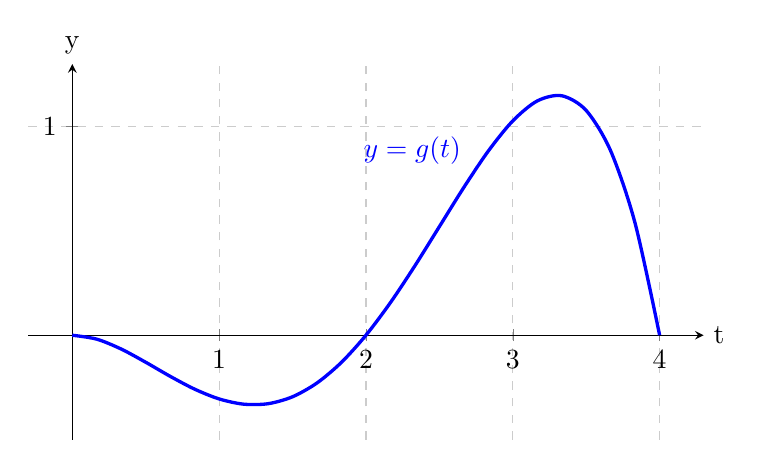
\begin{tikzpicture}
			\begin{axis}[
				xmin=-0.3, xmax=4.3, ymin=-0.5,ymax=1.3,    
				axis lines =middle,
				xlabel={t}, ylabel={y}, 
				every axis y label/.style={at=(current axis.above origin),anchor=south},
				every axis x label/.style={at=(current axis.right of origin),anchor=west},
				xtick={0,...,4}, ytick={0,..., 1},
				grid=major, width=4in, height=2.5in,
				grid style={dashed, gray!40} ,
				]
				
				\addplot[color=blue, very thick, smooth, domain=0:4]{-(0.006182)*x^2*(x-2)*(x-4)*(x+15.469)} node[pos=0.6, above left]{$y=g(t)$};

			\end{axis}
		\end{tikzpicture}
	\end{center}



\begin{enumerate}
  
  	%part a
    \item
      Circle the correct statement about $A(2)$.
      \begin{enumerate}
        \item $A(2) = 0$;
        \item $A(2) > 0$;
        \item $A(2) < 0$;
        \item none of the previous answers.\\ \\
      \end{enumerate}
      
      %part b
    \item
      Circle the correct statement about $A(3.8)$.
      \begin{enumerate}
        \item $A(3.8) = 0$;
        \item $A(3.8) > 0$;
        \item $A(3.8) < 0$;
        \item none of the previous answers.\\ \\
      \end{enumerate}
      
	%part c
    \item
      Circle the correct statement about $A'(3.8)$.
      \begin{enumerate}
        \item $A'(3.8) = 0$;
        \item $A'(3.8) > 0$;
        \item $A'(3.8) < 0$;
        \item none of the previous answers.\\ \\
      \end{enumerate}
      
%part d
    \item
      Find the solution of the following initiual value problem: $y'(x) = g(x)$ and $y(0) = 2$.
      \begin{enumerate}
        \item $y(x) = g(x)$;
        \item $y(x) = g(x) + 2$;
        \item $y(x) = A(x)$;
        \item $y(x) = A(x) + 2$;
        \item $y(x) = g'(x)$;
        \item $y(x) = g'(x) + 2$;
        \item none of the previous answers.\\ \\
      \end{enumerate}
      
%part e
    \item
      Find the expression for $\int_0^4 |g(t)| \d t$.
      \begin{enumerate}
        \item $A(4)$;
        \item $A(2) - A(4)$;
        \item $A(4) - A(2)$;
        \item $A(4) - 2 A(2)$;
        \item none of the previous answers.\\ \\
      \end{enumerate}
      
%part f
    \item
      Find the midpoint Riemann sum for the function $g$ on the interval $[0, 4]$ with $n = 2$ (the number of subintervals).
      \begin{enumerate}
        \item $g(1) + g(3)$;
        \item $g(0) + g(2)$;
        \item $g(2) + g(4)$;
        \item $2g(1) + 2g(3)$;
        \item $2g(0) + 2g(2)$;
        \item $2g(2) + 2g(4)$;
        \item none of the previous answers.
      \end{enumerate}
      
\end{enumerate}

\end{problem}

\end{document}
